%%%%%%%%%%%%%%%%%%%%%%%%%%%%%%%%%%%%%%%%%%%%%%%%%%%%%%%%%%%%%%%%%%%%
% Basic Informations
%%%%%%%%%%%%%%%%%%%%%%%%%%%%%%%%%%%%%%%%%%%%%%%%%%%%%%%%%%%%%%%%%%%%

\chapter{Basics}\label{Basics}
% todo explain EA, Gene, Genome, Allel. 
\section{TODO}
-> neural networks

\section{NEAT}\label{NEAT} % todo in ea section packen... und mit em deitschen ea paper zitieren. Biologisch eh nicht ganz korrekt
\Gls{neat} (\cite{NEAT}) is an neuroevolution method that genetically encodes and evolves weights and topologies of neural networks. \gls{neat} stands out from other neuroevolution algorithms by meaningful crossovers in disparate ANN topologies, protection of topological innovations and a efficient search by a stepwise increasing search space. (TODO cite some). Furthermore \gls{neat} is well suited for reinforcement learning problems. 
\subsection{biological basics} 
% maybe definitions are better ask %MKK zitieren %% todo fachwerk aus bib
The whole inheritable information needed to create a new organism is called genome. A genome consists of genes which are responsible for the expression of specific features. Genes that express same features with  different characteristics are called alleles. Assuming the eye colour is expressed by one gene.  Variations of this gene which lead to different eye colours are alleles. (TODO find proven example with one gene, TODO find source)
\subsection{Evolutionary algorithm} % Todo abkürzung EA
Evolutionary algorithms (EAs) (see generally \cite{book:IntroductionEA},\cite{book:IntroductionEA}) are algorithms that mimic the natural evolution process. That is simplified that only fittest organisms of a generation will survive. An EA maintains a group of solutions called a population. A solution in a population is called an individual. Each individual has a numerical fitness value that determines how good this solution is. An individual is represented by a code also called genome. During the run of an EA a genome of an individual undergoes several variation operations. One typical operations are mutations, where parts of the genome are changed randomly. Cross Over as an other typical operation exchanges parts of the genome of two individuals. Usually an EA performs those operations to generations and only the fittest childs are s taken over into a new generation. The function giving the fitness of an individual is called objective function. EAs are mainly used to find good local maxima of objective functions that are either unknown or not analytical differentiable and not solvable with numerical methods like gradient descends.  (TODO nachlesen vergleichn script zell). A  typical EA solution process can be illustrated as follows:
%\begin{algorithm}
%	\LinesNumbered
	\SetCommentSty{text} 
\begin{algorithm}[h!] % or H with float
   \TitleOfAlgo{Exemplar EA}
	choose strategy parameters\;
	create initial population P(0)\;
	$t \gets 0$\;
	evaluate fitness of the initial population\;
	\While{termination condition not reached}{
		$t \gets t+1$\;
		apply variation operations \tcp*[r]{e.g. mutation, cross over}
	    evaluate fitness of new individuals\;
		create new population P(t)\;
	}
 	output results;
 	
	%\caption{How to write algorithms}
\end{algorithm}
%\end{algorithm}...
TODO typischer evolutionszykel erklären.


\subsection{operating principle} 
The genetic basic of \gls{neat} is a direct encoded genome, which contains connection and node genes. Each node gene evolves a neuron while each connection gene represents a weighted and directed connection between two neurons. A node gene contains it's identification number and it's type. Possible types are Input, Output and Hidden. A connection gene encodes its connection by referring to two node gene identification numbers. In addition a connection gene contains its weight, an expression flag and an innovation number. The expression flag indicates whether the expression gets realised or not. The innovation number is the fixed identification number of a connection gene. Alleles of a connection gene share the same node genes and innovation number but can have different weight and expression flag values. Every time a new neuron gene or connection gene is created a global counter number is increased by one and than used as the new innovation number. In the case that the same connection gets created in two different offsprings of a generation they get the same innovation number assigned. This only applies if it happens in the same generation. Thus one gene can only evolve in one particular generation. As a result the innovation number assures that connection genes with the same innovation number connect the same nodes but not all connection genes connecting the same nodes have the same connection number.(this represents the biological fact, that the same feature can be expressed by different genes.). An example for a NEAT genome is depicted in figure \ref{fig:neatgenome}.\\
Three types of mutation are realized. A \textit{weight mutation} mutates each weight mutates with the same probability. New connections are added by the add connection mutation. Thereby two unconnected cells are randomly chosen and connected by a new connection gene with a random weight. A new cell mutation splits an existing connection by placing a new node between the two former connected nodes. This is realized by disabling the old connection gene and the creation of two new connection genes and one new node gene. One connection gene connects the input node with the new node and gets its weight set to the value of the former connection. The other connection gene is connects the new node with the output node of the former connection and gets its weight set to one. This expression of weights leads to an minimized initial effect of a mutation. Two exemplar mutations are displayed in figure \ref{fig:neatmutations}.\\
In? a cross over at first a synapsis is done. This means that all connection genes of two individuals are lined up. Genes that have the same innovation number are called matching genes. Genes of one individual which innovation numbers are inside the range of the other individual matching genes' innovation numbers are called disjoint genes. Innovation numbers outside the range of the other individual matching genes' innovation numbers are called excess genes. The child's genome is created by selecting one gene randomly out of each tuple of matching genes, disjoint and access genes are taken from the more fit parent. With a preset probability a disabled gene can be enabled again when it is disabled in both parents. By crossing over only connections and no whole substructures of the network (like other approaches do  TODO find one vorlesung Zell trees), it is ensured that a new proper artificial neural network is created. 
An exemplar cross over of two individuals with the same fitness is shown in figure \ref{fig:neatcrossover}. \\
Specitation: 
Based on empirical evidence insertion of new structures into a network leads at first to a decrease in fitness. Thus its unlikely that the individual can compete against others in this generation and will be distinct. A new structure needs some time to adapt its weights in a way that the new structure is beneficial. Thus specitation also known as niching is implemented in NEAT to protect new structure. Similar individuals are put in their own species. Members of a species are primarily competing against each others. That means artificial neural networks with similar structures are primarily competing against each other. To determine to which species an individual belongs the following distance measurement between two aligned individuals is used:
\begin{equation*} 
\delta = \dfrac{c_1E}{N}+\dfrac{c_2D}{N}+c_3*\overline{W}.
\end{equation*}
Where $E$ is the number of excess genes and $D$ the number of disjoint genes. $\overline{W}$ is the average of weight differences of all matching genes. The normalization factor $N$ is the number of genes of the larger genome. $c_1$,$c_2$,$c_3$ represent scaling factors. 
In detail a ordered list of species is given. For the next generation one representative individual is randomly chosen out of each species. Each member $m$ of the next generation is compared consecutively to these representatives. If the distance measurement $\delta$ is smaller than a fixed threshold $\delta_t$, $m$ is put into the species of the representative. If $m$ is not compatible to any representative a new species with $m$ as its representative is created. This way assures disjunct species.
To prevent that one species takes over the entire population explicit fitness sharing (TODO link Golsberg and Richardson 1987) is used. For each individual $i$ its adjusted fitness $f_{i}^{'}$ is calculated the following way:
\begin{align*} 
f_{i}^{'}&=\dfrac{f_i}{\displaystyle\sum_{j=1}^{n} sh(\delta(i,j)) }\\
sh(i,j) &= \begin{cases}
1 & \quad \text{if } \delta(i,j) < \delta_t \\
0 & \quad \text{if } \delta(i,j) \geq \delta_t
\end{cases}
\end{align*}
Where $f_i$ is the fitness of $i$, $\delta(i,j)$ the distance between individual $i$ and $j$. And $sh$ a sharing function that determines whether $i$ and $j$ are in the same species.
As a result under the assumption that the fitness function has no plateaus at local maxima the shared fitness of species members is decreased if the species gets larger. Every species produces a number of offsprings $NO$ proportional to the sum of adjusted fitnesses $f_{i}^{'}$ of its members. The total amount of offsprings is limited by the maximum population size $P$ and the number of individuals that are taken over directly from the last generation $L$.
\begin{equation*} 
NO(s) = (P-L)\cdot\dfrac{\displaystyle\sum_{\forall i \in s} f_{i}^{'}}{\displaystyle\sum_{\forall i } f_{i}^{'}}
\end{equation*}
  %TODO bei zell im script nachlesen -> verbessern.
\\ NEAT starts with a minimal structure. That is, each input neuron and one optional bias neuron is connected with each output neuron. There are no hidden neurons. Starting with a minimal structure leads to an efficient search. Since add node mutations and add connection mutations are rare compared to weight mutations the search space is increased slowly. The search space consists of one dimension for each weight and one dimension representing the number of neurons. That means starting with a minimal network networks with increasing complexity are considered as solution for the problem.


 
  
  
\begin{figure}[tb]
	\centering
	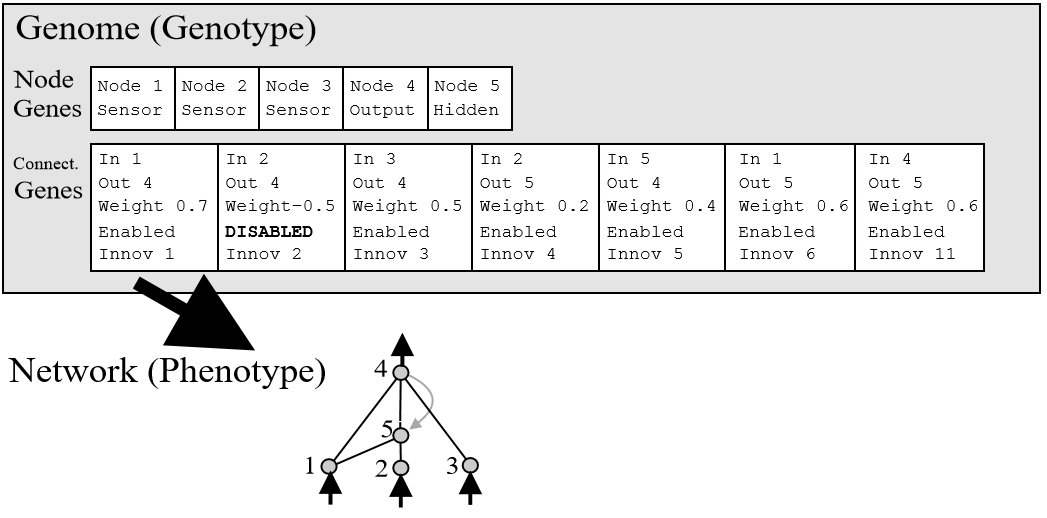
\includegraphics[width=0.7\linewidth]{figures/NEAT/NEATGenome}
	\caption[NEAT genome]{NEAT genomes consist of two type of genes: node genes displayed in the first row and connection genes displayed in the second row. Each node gene has an identification number (first element) and one of three types: sensor (input), output and hidden. A connection gene contains its input and output node, a weight, an expression flag and a innovation number. Underneath the genome the resulting network is displayed. The numbers are identical to the node IDs. Enabled connections are displayed black. Disabled connections are shown grey. \cite[p. 106]{NEAT} }
	\label{fig:neatgenome} % TODO wirklich so ausführlich wiederholen notwendig?
\end{figure}
  
  
  
\begin{figure}[tb]
	\centering
	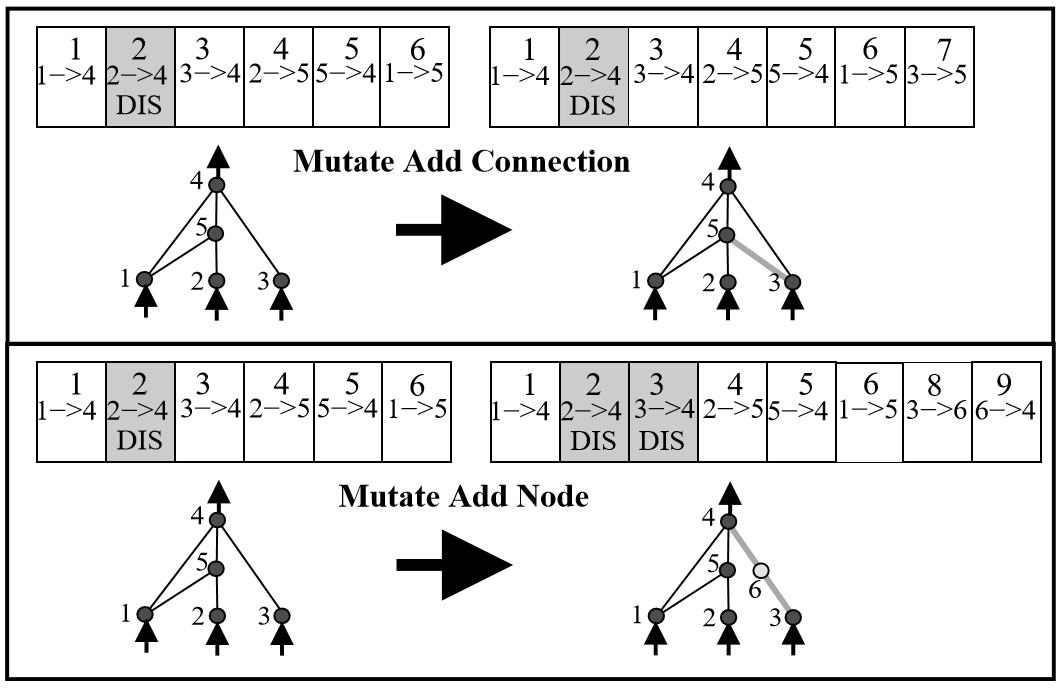
\includegraphics[width=0.7\linewidth]{figures/NEAT/NEATMutations}
	\caption[NEAT mutations]{At the top a add connection mutation is displayed. The unconnected nodes 3 and 5 are chosen randomly. Then a connection gene between  those nodes is created. The global innovation counter number is increased by one (from 6 to 7) and allied to the new connection gene.\\
	At the bottom a add node mutation is displayed. Connection 3 is randomly chosen and gets disabled. Next a new node gene with ID 6 is created. Then fist new connection gene connecting  node 3 and 6 with innovation number 8 and a second connecting node 6 and 4 with innovation number 9 is created. \\
Note that only connection genes are displayed. The top number in each gene is its innovation number followed by the node it connects and the expression flag.
Node genes are not depicted.
\cite[p. 107]{NEAT}}
	\label{fig:neatmutations}
\end{figure}
  
  
  
\begin{figure}[tb]
	\centering
	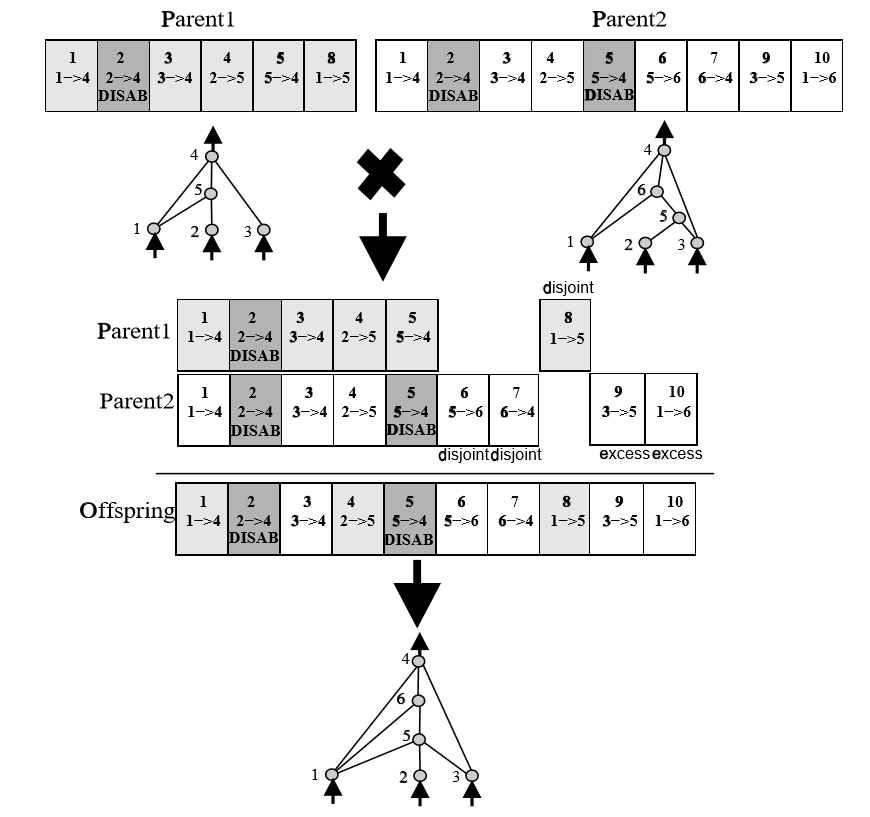
\includegraphics[width=0.7\linewidth]{figures/NEAT/NEATCrossOver}
	\caption[NEAT cross over]{Two individual's connection genes and their corresponding networks are displayed at the top. Underneath this two genomes got aligned. All connection genes with same innovation numbers are displayed opposite each other. Those are matching genomes. All connection genes of one individual that are in the range of the other individual's connection gene are marked as disjoint. Connection genes that are outside the range of the other individual's connection gene are marked are marked as excess. The offspring's connection gene consists of one randomly chosen connection gene out of each matching gene. In this example the fitness of both parent individuals is equal. Thus all excess and disjoint connection genes are chosen. If the fitnesses would differ the excess and disjoint connection of the more fit parent are taken over.\cite[p. 109]{NEAT}}
	\label{fig:neatcrossover}
\end{figure}
  
  
Neuroevolution is a machine learning technique that evolves weights and topology of artificial neural networks by means of evolutionary algorithms. 

TODO: explain 
Neuroevolution
evolutionary algorithm


"Neuro-evolution of augmenting topologies (NEAT) is a method for genetically encoding and evolving the architecture and the weights of neural networks "

\section{HyperNEAT}\label{HYPERNEAT}
 While NEAT (see \ref{NEAT}) works well on considerably small networks it's performance decreases for large networks greater several hundred neurons. (TODO find paper with prove.). With this amount of neurons the search space get's to big, thus finding a solution with NEAT gets computational expensive. 
 Hypercube-based NeuroEvolution of Augmenting Topologies (HyperNEAT) (TODO cite) addresses this problem searching in a space of spatial connection patterns instead of searching in a space where each single connection is considered. As a result connections of large ANNs can are indirect encoded by a single multidimensional function. It was even shown by (TODO cite) that on the basis of such a function it is possible to scale the amount of neurons of the found network leading only to minor changes in functionality. A further fundamental principle of HyperNEAT is, that the position of neurons in space are included into the search space.(TODO cite). Relationships between neurons are described by their distance. Similar neurons are placed next to each other. The indirect encoding is inspired by the biological fact that $30,000$ genes  (cite hneat paper p 4 reffs) encode the human brain with approximately $100 \cdot10^9$ neuron connections.
 
 The function $f$ describing the spatial pattern and the function  $w$ describing the resulting connection weights are defined as follows: 
\begin{align*} \label{HyperNEatFunction}
 f&\colon \mathbb{R}^{2n} \to [l,u], \quad  p_{1_1},\ldots,p_{1_n},p_{2_1},\ldots,p_{2_n} \mapsto f(p_{1_1},\ldots,p_{1_n},p_{2_1},\ldots,p_{2_n})\\
 w&\colon \mathbb{R}^{2n} \to [0,w_{max}] \text{ with: }\\
 w&(p_{1_1},\ldots,p_{2_n})=\begin{cases}
 \dfrac{f(p_{1_1},\ldots,p_{2_n})-\theta_c}{u-\theta_c} \cdot w_{max} & \quad \text{if } f(p_{1_1},\ldots,p_{2_n}) \geq \theta_c \\
 0 & \quad \text{if } f(p_{1_1},\ldots,p_{2_n}) < \theta_c \\
 \end{cases}\\
 \text{w}&\text{ith } l\leq \theta_c \leq u  
 \end{align*}\\
 Where $\mathbb{R}^n$ is the spatial space of the neuron. Thus $2n$ is the dimension of the connection space a hypercube, where one point describes the connection between two neurons. $l$ and $u$ are the boundaries of the connection space. $p_1$ and $p_2$ describe the neuron coordinates of two neurons in an n-dimensional space. The maximal weight is described by $w_{max}$. $\theta_c$ is called the connection threshold (TODO name, bzw hat keinen namen).
 Note that this mathematical definition has been created on the verbal description of Kenneth... (TODO cite). Described in words , the coordinates of two neurons are given to $f$. If $f$'s output is higher than $\theta_c$ a connection is created and it's weight is $f$'s output scaled between $0$ and $w_max$.\\
Description of f:
f is calculated by a Compositional Pattern Producing Network CPPN. To prevent confusion f is referred to as CPPN further on. A CPPN is a network where each node is a function out of a pool of basic functions. It works like an ANN, where the activation functions are replaced by a function out of the pool of basic functions.typical used basic functions are sinusoidals, lines and gaussians. An exemplar CPPN can be seen in figure (\ref{cppn}).
Since CPPNs are identical to ANN, they get evolved by NEAT. That ensures that HyperNEAT's search starts initially with simple connection patterns, whose complexity gets increased during the search. 
In HyperNeats terminology like in NEAT the network describing the CPPN is named the genome. The placement of neurons of the resulting ANN in the neuron space is called the substrate configuration. The resulting network is called the substrate. Similar neurons should be placed next to each other, since they will get similar connection patterns than.Exemplar substrates are shown in figure \ref{fig:substrates} \cite{GeometrySensitvityHyperneat}  proves empirically  that giving geometric information about the problem improves the search, however choosing a random geometric representation works worse but still good solutions can be found. Furthermore they show that the dimensionality of the input space has a influence on the result.  Thus also problems where the geometric information is unknown are solvable.  So to determine the weight of the connection of two neurons, their positions are applied as input parameters to the CPPN and like described in \ref{HyperNEatFunction} the weight value is determined. This process is also depicted in \ref{fig:querysubstrate}. Note that there are two different ANNs in HyperNEAT: the CPPN describing a function in the connection space and the resulting ANN which connections are defined by the output of the CPPN. 
To sum up the algorithm works as follows:

	\SetCommentSty{text} 
\begin{algorithm}[h!] % or H with float
	\label{HyberNEATAlgorithm}
	\TitleOfAlgo{HyperNEAT algorithm}
	choose strategy parameters\;
	define a substrate configuration C \;
	create initial population P(0) with minimal CPPNs and random weights\;
	$t \gets 0$\;
	evaluate fitness of the initial population\;
	\While{termination condition not reached}{
		$t \gets t+1$\;
		\ForAll(\tcp*[f]{genome = CPPN}){genomes in P(t) }{ 
		 \ForAll{pairs of nodes in C }{
			apply node positions to CPPN and determine the connection weight for the connection between the pair of nodes\; 
		}
		Determine fitness of created ANN\;
	}
		 new population P(t) with NEAT\;
	}
	output best CPPN;
	%\ similar in modularity paper
	%\caption{How to write algorithms}
\end{algorithm}

\begin{figure}[tb]
	\centering
	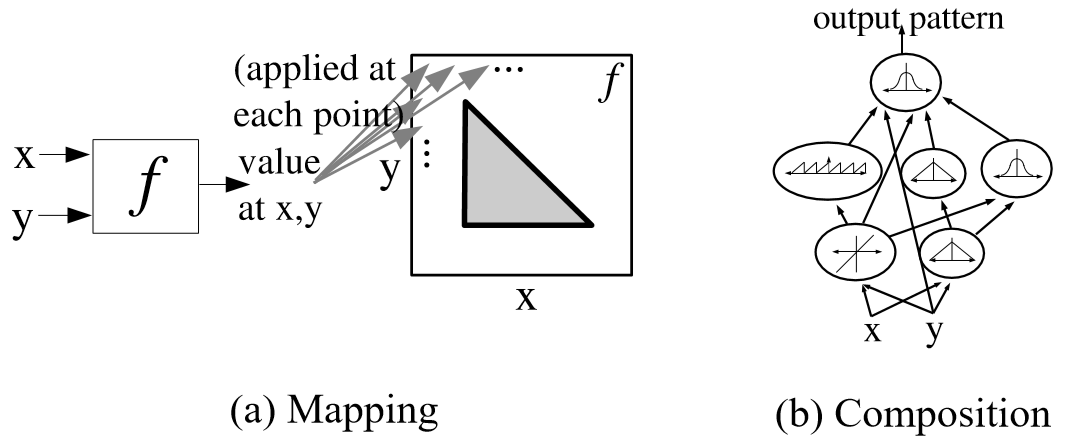
\includegraphics[width=0.7\linewidth]{figures/HyperNeat/CPPN}
	\caption[Exemplar CPPN]{(a) The mapping of a function f from a two dimensional connection space to a one dimensional spatial pattern. x and y are the positions of two neurons. (b) f's internal structure called a CPPN is shown. The output is a composition of different basic functions in a network. The connections in the CPPN are weighted such that the output of a function by the weight of it's outgoing connection. \cite[p. 5]{HyperNEAT}}
	\label{fig:cppn}
\end{figure}

\begin{figure}[tb]
	\centering
	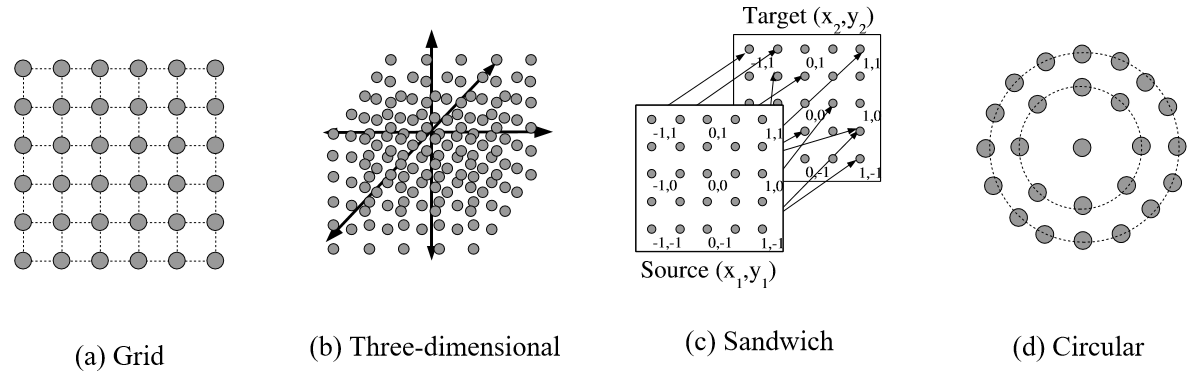
\includegraphics[width=0.7\linewidth]{figures/HyperNeat/Substrates}
	\caption[Exemplar Substrate Configurations]{ Examples of how to define a substrate configuration. That is how to arrange the position of neurons. They can be of different dimensions and described by different coordinate systems. (a),(b) and (c) are in Cartesian coordinates while (d) is represented in polar coordinates. (a) and (d) are one dimensional while (b) is three dimensional. (c) is an implicit three dimensional case, where the third dimension is ignored. In this case all input neurons lay on a different layer in 3D space than the output neurons. Note that self linked neurons are not possible in this scenario. Substrates describe the geometric relationship of neurons, so different substrates are suited for problems with different geometric properties.
	\cite[p. 11]{HyperNEAT}}
	\label{fig:substrates}
\end{figure}



\begin{figure}[tb]
	\centering
	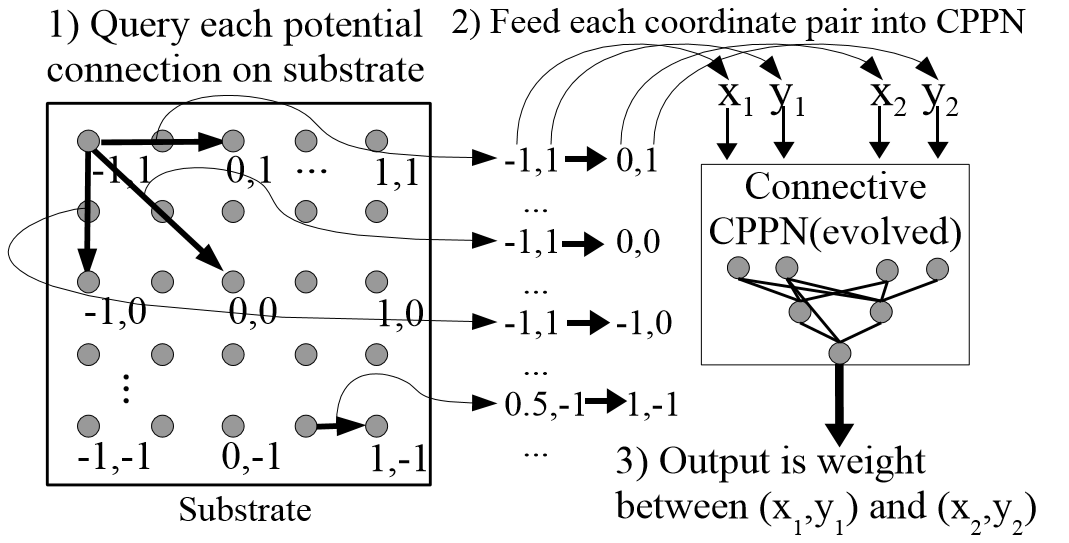
\includegraphics[width=0.7\linewidth]{figures/HyperNeat/QuerySubstrate}
	\caption[ANN creation with HyperNEAT]{This figure shows how a ANN is created by HyperNEAT. The coordinates of each pair of nodes (potential connection) are applied to the CPPN. A pair of nodes is depicted by a black arrow. If the CPPN's output is higher as a defined threshold (not depicted) a weighted connection between those two nodes is created. In this example a two dimensional grid substrate and thus a CPPN with four inputs is used. 	\cite[p. 9]{HyperNEAT} }
	\label{fig:querysubstrate}
\end{figure}


\begin{figure}[tb]
	\centering
	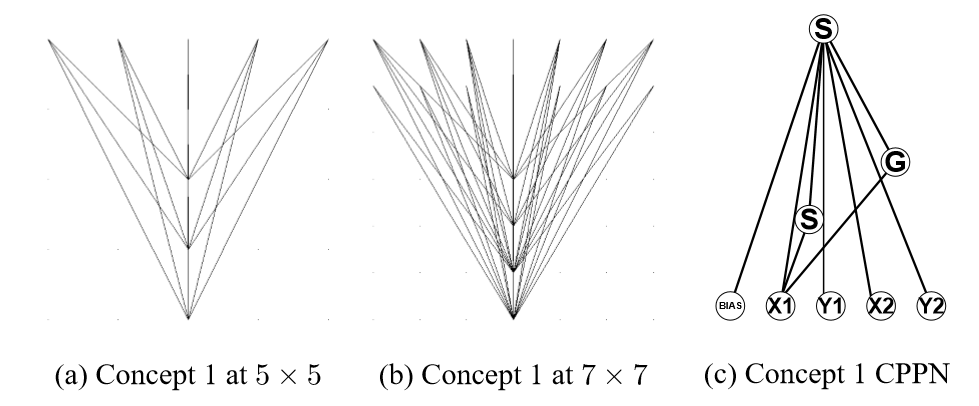
\includegraphics[width=0.7\linewidth]{figures/HyperNeat/scaling}
	\caption[Exemplar substrate scaling]{ The spatial pattern produced the CPPN on the right (c) can be queried by different substrates. (a) shows the resulting network of a 5 x 5 grid substrate and (b) the resulting network of a 7 x 7 grid substrate on the same space. From (a) to (b) the substrate was even scaled by factor $1.4$.  \cite[p. 14]{HyperNEAT}}. The CPPN activation functions are denoted by G for Gaussian and S for sigmoid.
	\label{fig:scaling}
\end{figure}

Scaling:\\
 \cite{HyperNEAT} and \cite{HyperNEATOctobusArm} argue that the spatial pattern produced by a CPPN encodes a general connectivity concept. Based on this statement they show empirically that the resolution of a substrate configuration can be changed to vary the size of the resulting ANN with only minor influences on the result. For example instead of an $5x5$ grid substrate configuration one could scale the substrate configuration to a $7x7$ grid substrate applied to the same space (e.g $[0,1]$). This process is further on referred as substrate scaling. One benefit of substrate scaling is, that one can scale the resulting with use of the same substrate without further evolution needed. Example solution of a scaled substrate configurations are shown in figure \ref{fig:scaling}.
 
 CPPN configuration variation: \\
 \cite{HyperNEATOctobusArm}, \cite{HyperNEATLeo},\cite{HyperNEATEvolveLearningRules} and \cite{HyperNeat1DSubstrates} varied the number of inputs and outputs of the CPPN to encode further information than the neuron position. \cite{HyperNEATLeo} decouples the weight and the expression of a connection. He defines with the value of a second output whether the connection is evolved or not. One other variation from \cite{HyperNEATOctobusArm}  is two have three layered sandwich substrate configuration where the second CPPN output defines the connections between the second and third layer.\cite{HyperNEAT} adds an additional input node to additionally decode the distance between the geometric distance between the two nodes. Further on one can use a additional bias neuron wit a constant input as input neuron as \cite{HyperNEATEvolveLearningRules} did. TODO draw own picture with those variations.  \cite{HyperNEATLeo} states that Hyperneat "tends to generate fullyconnected networks" and shows that due to the separation of weight encoding and connectivity expression less connected modular networks can evolve.
 

  
 
 

 Wichtig, gutes zitat irgendwo verwenden:
 \cite{HyperNEATLeo} states that Hyperneat "tends to generate fullyconnected networks"

 Scaling: TDDO 
 CPPN configurations: multiple input, outputs
 Modulationary CPPNs:
 
 
 zitiere checkers game, robot arms, b

TODO mention much lower search space in cppn.


substrate = output of cppn
or substrate = placement of neurons.
or substrate = resulting network !!
Ok last one gives most sense!!

TODO draw retina example.

-> senstifity to chosen geometrie -> Paper (The Sensitivity of HyperNEAT to Different Geometric Representations of a Problem)

Hypercube-based NeuroEvolution of Aug
menting Topologie
\subsection{Basic HyperNEAT}
\subsubsection{Scaling}
\subsubsection{Modulation}
\subsection{ES HyperNEAT}\label{ES_HYPERNEAT}

\section{Motorcortex Model}\label{MotorCortex_Model}